\chapter{Background}
\label{chap:Background}

\section{Messages}
\label{sec:Messages}

In today's interconnected world, computer programs rarely exist in a vacuum.
Rather, they form one small part of a much larger \gls{soa} -
consisting of multiple services, jobs and scripts, all exchanging information in
the form of messages. These messages may adhere to a standard data-interchange
format (for example, \gls{json}). They may correspond to an agreed upon
specification (for example, \href{https://goo.gl/rjuP4C}{IEEE 1671-2010}).
Or they may simply be blobs of binary information transmitted over the network -
completely subject to the interpretation of the sender and received.
At a fundamental level, though, a message is simply a collection of bytes, to be
transmitted from point A, to point B.

\section{Message Brokers}
\label{sec:brokers}

\begin{figure}[ht]
  \centering
  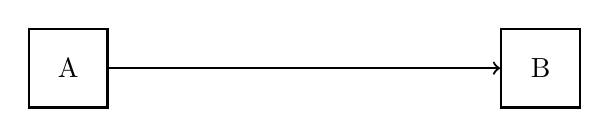
\begin{tikzpicture}[thick]
  \node(A) [draw,rectangle,minimum width=1cm,minimum height=1cm]{A};

  \begin{scope}[xshift=6cm]
    \node(B) [draw,rectangle,minimum width=1cm,minimum height=1cm]{B};
  \end{scope}

  \draw[->] (A) edge (B);
\end{tikzpicture}

  \caption{Two services, A and B, directly exchanging messages}
  \label{fig:tikz:directMessaging}
\end{figure}

To understand the role message brokers typically play in \glspl{soa}, we first
examine the simplest method of transmitting bytes between two applications -
directly transmitting messages between two applications (shown in
Figure~\ref{fig:tikz:directMessaging}).

In this example, the application 'A' wishes to transmit a simple message (a
sequence of bytes) to application 'B', and does so in the simplest method
possible. This could involve making an \gls{rpc}, opening a Unix/\gls{tcp}
socket, or making a HTTP web request - for the purposes of this illustration the
exact mechanism by which bytes are transferred is unimportant, the fact that the
transfer takes place \emph{directly} between the two parties is all that
matters.

\subsection{Queues}
\label{sub:Queues}

Brief overview of the features/operation of a queue, in relation to a message broker.


\subsection{Topics}
\label{sub:Topics}

Brief overview of the features/operation of a topic, in relation to a message broker.

\subsection{Existing Brokers}
\label{sub:Existing Brokers}

Brief overview and comparison between some existing commercial/open-source
implementations, and their features.


\section{Project Requirements}
\label{sec:SLA/QoS Specification}

A message-broker is rather an unusual piece of software, due to the fact that is has very few functional requirements.

\subsection{Failure Handling}
\label{sub:Failure Handling}

The issue with gracefully handling communications failure in distributed systems
was illustrated in a 1988 paper by Xerox employees
Andrew Birrell and Bruce Nelson\cite{Birrell:1988:IRP:59309.59336}. They identified
three different semantics with which \glspl{rpc} could be executed:

\begin{description}
  \item[Exactly once] \hfill \\
    The ideal scenario is one in which messages are passed to their destination
    once, and exactly once. Typically, when failure does not occur during a
    message transfer this is trivial to assert - simply receiving an acknowledgement
    from the recipient of the message confirms this to be the case.
    Unfortunately, the same cannot be said when a response is not received from
    the recipient, for whatever reason (link failure/machine failure etc.).
    This is a typical illustration of the
    'Two Generals Problem'\cite{Gray:1978:NDB:647433.723863} - and is extremely
    difficult to guard against. As a result - most messaging systems adopt one
    of the following behavioural models in the event of failure.
  \item[At most once] \hfill \\
    In the event that a message is lost without acknowledgement - no attempt is made
    to redeliver the message. This is used in situations where duplicated messages
    pose a risk to overall system integrity - for example in most financial systems.
  \item[At least once] \hfill \\
    In the event that a message is lost without acknowledgement, attempts to
    redeliver the message continue until successful receipt is acknowledged.
    This is typically used in situations where message delivery is deemed more
    important than message uniqueness/ordering. For example, if the unacknowledged
    message is intended to trigger a cache refresh in the recipient system - the
    fact that the refresh may occur multiple times may be insignificant next to
    the risk that the refresh does not happen at all.
\end{description}

\subsection{Network Bandwidth Utilization}
\label{sub:Network Bandwidth Utilization}

In many situations (and in \gls{iot} devices in particular) network bandwidth is
a limiting resource. Message compression can be used in certain situations to
reduce overall bandwidth utilization of the broker - at the cost of increased
computational load on both the broker and consumer.

\subsection{Network latency}
\label{sub:Network latency}

Devices experiencing high degrees of network latency can have tremendous impact
on the overall \gls{rtt} of a given message. This can be compensated for through
intelligent packet stuffing (such as Nagel's algorithm)/jumbo frames (if supported)
by the network - all of which reduce the amount of overhead experienced by each
message.

\subsection{Network packet loss}
\label{sub:Network packet loss}

On networks experiencing a high rate of packet loss - error correcting protocols
like TCP can help ensure packet delivery at the IP layer. Additionally,
check-summing the messages can help guard against message corruption through lost
packets.

\subsection{Message power cost}
\label{sub:Message power cost}

Especially relevant for \gls{iot} and low-power devices - the amount of power
consumed whilst exchanging messages (which is directly linked to the number of
CPU cycles required to transmit/receive each message) can be an important
consideration when designing an applications. Message attributes which can
affect this include:

\begin{itemize}
  \item Message compression
  \item Message size
  \item IP Protocol
  \item Network conditions (requiring re-transmits/computing checksums etc.)
\end{itemize}

\subsection{Message throughput}
\label{sub:Message throughput}

Finally - the most obvious performance metric of a broker - the number of messages
it can process per second. This is impacted by all of the above requirements,
and can be maximized through the use of small, cheap messages, with as little
overhead as possible. Network protocol can make a large difference here - with
something like UDP being extremely cheap to send over the wire
(if inherently unreliable).

\section{GoLang}
\label{sec:GoLang}

\todo[inline]{Overview of GoLang}

\subsection{What is GoLang?}
\label{sub:What is GoLang?}

\todo[inline]{History/Purpose/Development}

\subsection{Concurrency vs Parallelism}
\label{sub:Concurrency vs Parallism}

\todo[inline]{Async IO vs multiple threads}

\subsection{Why do we need concurrency?}
\label{sub:Why do we need parallism}

\todo[inline]{Message broker functions - blocking vs non-blocking IO}

\subsection{Concurrency in GoLang}
\label{sub:Concurrency in GoLang}

\todo[inline]{GoRoutines/Channels etc.}
